\newpage
\chapter{Efficient Active-Lane Consolidation}
\label{chap:approach}

%Make sure that the heading of a chapter is a the top of the page.
%Also you should switch from \section to \chapter

This section presents an ALC design that addresses key limitations in Praharenka \etal's initial design\cite{praharenka_vectorizing_2022}. After a review of the original ALC design (\rsec{original-alc}), \rsec{gathers-scatters-are-bad} presents evidence that the higher-than-anticipated cost of the gather/scatter instructions renders Praharenka \etal's ALC ineffective.
The approach proposed in this work to eliminate gather/scatter instructions is presented in \rsec{alc-data-permutation}.
Lastly, \rsec{single-if-statement-approach} describes a novel algorithm that extracts the best of both ALC and control-flow linearization in a common case when loops have only a single \textbf{control-flow-divergent path} (\acrshort{cfdp}).

\section{Original ALC Design}
\label{sec:original-alc}

\begin{figure*}[t]
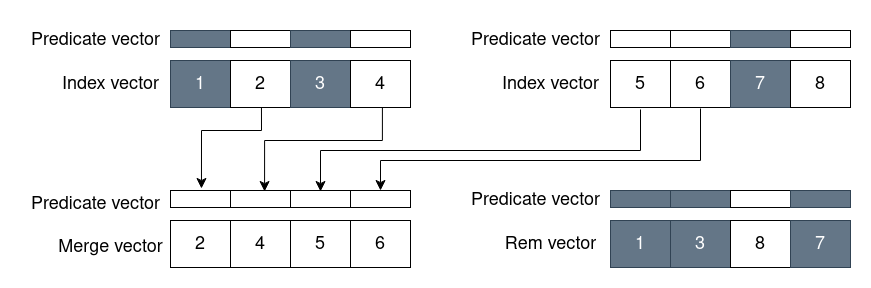
\includegraphics[width=\textwidth]{Figures/03-approach/Permutation.png}
\centering
\caption{Index Permutation: inactive elements are shown by gray color, while active elements are white. Given two vectors containing loop indices and their corresponding predicates, Permutation algorithms merges active elements into \emph{merge} vector and puts all remaining ones into \emph{Rem} vector.}
\label{fig:permutation}
\end{figure*}


Praharenka \etal propose two variations of ALC: \unrollALC and \iterALC.
In both versions, ALC is applied after \ifconversion.
In the \unrollALC, the \ifconverted and vectorized loop is unrolled once and two index vectors are formed, one for each iteration of the loop before unrolling.
Each index vector is initialized such that each lane contains the value of the loop's induction variable of each scalar iteration.

At the heart of ALC is the \textbf{Permutation} algorithm which tries to create a uniform vector with minimal overhead from two vectors and their corresponding predicates. \rfig{permutation} shows how active elements of two index vectors are merged together to form a uniform vector.

In Praharenka \etal's work, the path that is most likely to be taken across all iterations of the loop is chosen for consolidation based on profiling information.
Then two predicate vectors are formed by evaluating the condition to execute that path. After doing permutation, all vector operations in the consolidated path operate with uniform vectors without predication.
This work focuses on cases with small ($< 3$) paths and thus consolidation is applied to all paths.

Once the predicates are formed, the index vectors are permuted such that all active lanes are consolidated into a \emph{merged vector} \vM.
The inactive lanes are kept in a \emph{remainder vector} \vR.
Finally, if the \vM is uniform, then the consolidated uniform path is executed.
Otherwise, the \ifconverted path is executed.
The main difference between \unrollALC and \iterALC is that, in \iterALC, the \ifconverted and vectorized loop is not unrolled.
Instead, the active lanes from multiple iterations are merged into \vM until \vM is a uniform vector. 
Only then the consolidated uniform path is executed.
\iterALC works well for loops with a conditional that contains vectorizable code in both the then and the else block.
In this case, \code{then} lane are consolidated into \vM, and \code{else} lane are consolidated into \vR.
Whenever either \vM or \vR is full, the corresponding code can be executed in a uniform vector.


In both versions, any data that is dependent on the loop indices --- e.g. arrays $a$, $b$, and $c$ in \rlst{simple-loop} ---, are loaded using gather-load instructions because a consolidated vector might contain non-consecutive indices.
A gather-load instruction loads data from (potentially) non-consecutive addresses calculated by adding a base-pointer operand to each index in the index-vector operand.

Similarly, any write-back to memory needs to be performed via scatter-store instructions, which also can write into non-consecutive memory addresses.
By design, the use of gather/scatter instructions is unavoidable in Praharenka \etal's ALC. In \rsec{gathers-scatters-are-bad}, experimental results show that gather/scatter instructions can render ALC ineffective on real hardware with SVE.

\rlst{simple-loop-alc} shows the loop in \rlst{simple-loop} after a version of iterative ALC is applied to it. The two paths inside the loop are consolidated. Once the permutation is done in each iteration of the loop. there will always be either a uniform active vector (\vM) or a uniform inactive vector (\vR). As a result, one of \Then or \Else blocks will be executed in each iteration with no predication. As discussed, every load and store operation inside \Then and \Else blocks are done through gather and scatter instructions.

\begin{center}
\begin{minipage}[t]{0.8\columnwidth}
\begin{lstlisting}[
escapechar=|,
language=C,
caption={ALC applied to the loop in \rlst{simple-loop}.}, label=lst:simple-loop-alc]
    /*Initialization*/
    idxM = index(0, VL);
    a_0 = vld(a[0]);
    b_0 = vld(b[0]);
    pred_M = a_0 < b_0;
    for (int i = VL; i < N; i += VL) {
         idxR = index(i, VL);
         a_i = vld(a[i]);
         b_i = vld(b[i]);
         pred_R = a_i < b_i;
         vM, vR, cond_M, cond_R =
          Permute(idx_M, idx_R, pred_M, pred_R);
         if(cntp(cond_M) == VL){
    /* execute if block without predication */
            b_v = gather(&b, vM);
            c_v = gather(&c, vM);
            mul_v = b_v * c_v;
            scatter(&a, vM, mul_v);
            idxM = vR;
            pred_M = cond_R;
         }else{
    /* execute else block without predication */
            a_v = gather(&a, remaining_vec);
            c_v = gather(&c, remaining_vec);
            add_v = a_v + c_v;
            scatter(&b, remaining_vec, add_v);
            idxM = vM;
            pred_M = cond_M;
         }
    }
}
\end{lstlisting}
\end{minipage}
\end{center}





\section{How Gather/Scatter Instructions Hurt ALC}
\label{sec:gathers-scatters-are-bad}

\begin{center}
\begin{minipage}[t]{0.8\linewidth}
\begin{lstlisting}[
style=code_snippet_style,
language=C,
caption={Simple conditional copy loop.},
label=lst:simple-cond-copy-loop]
for (int i = 0; i < n; i++) {
    if (cond[i]) {
        b[i] = a[i];
    }
}
\end{lstlisting} 
\end{minipage}
\end{center}

In order to understand the prohibitive overhead of gather/scatter instructions in ALC's performance, consider the simple loop in \rlst{simple-cond-copy-loop}.
The loop conditionally copies elements from array $a$ to array $b$, both are 32-bit integers.
An element $a[i]$ is copied to $b[i]$  if, and only if, the value in $cond[i]$ is true.
\rtab{gather-scatter-bad} shows performance metrics for different versions of the loop in \rlst{simple-cond-copy-loop}.
For the results in \rtab{gather-scatter-bad}, the \code{cond} array was initialized such that every other element has a \code{true} value ($50\%$ sparsity).
The results were obtained following the methodology in \rsec{methodology}.
Both \ALC and \ALCdp versions are generated by the compiler pass described in Chapter \ref{chap:alc-pass}.

\begin{table}[t]
\centering
\caption{Performance metrics when executing different versions of the loop in \rlst{simple-cond-copy-loop}: number of cycles to execute the loop (\textit{Total Cycles}), number of executed instructions (\textit{Num. Exec. Instructions}), cycles with no instruction completed (\textit{Stalled Cycles}), and cycles stalled due to memory operations (\textit{Memory Ops. Stalled Cycles}). Versions of the code: non-vectorized (\scalar), \ifconverted \& vectorized (\ifconv), \iterALC with gather/scatter instructions (\ALC), and \iterALC with data permutation and without gather instructions (\ALCdp).}
\label{tab:gather-scatter-bad}
\begin{tabular}{|p{2.7cm}|p{1.8cm}<{\centering}|p{2.1cm}<{\centering}|p{1.8cm}<{\centering}|p{2.7cm}<{\centering}|}
\hline
\makecell{Version/Metric} &
\makecell{Loop\\ Cycles} &
\makecell{Num. Exec.\\ Instructions} &
\makecell{Stalled\\ Cycles} &
\makecell{Memory Ops.\\ Stalled Cycles} \\ \hline
\scalar &    132M &  224M &    21M &  1.6M \\ \hline
\ifconv &    14M  &   14M &     9M &  1.2M \\ \hline
\ALC    &   220M  &   16M &   210M &  110M \\ \hline
\ALCdp  &    58M  &   63M &    38M &  1.3M \\ \hline
\end{tabular}
\end{table}

Unsurprisingly, all vectorized versions of the loop --- \ifconv, \ALC, \ALC  --- execute fewer instructions than the \scalar code.
Each vector instruction in the loop operates on 16 32-bit integers at a time ($VL = 512$ bits).
However, \ALC is more than $66\%$ slower than \scalar, even while it executes $14\times$ fewer instructions, because \ALC causes $10\times$ more stalls than the \scalar code.
More than half of the stalls are due to waiting for data from memory.
The main culprits are the gather/scatter instructions because they require multiple load/store ports instead of a single port as regular vector loads~\cite{A64FXmanual}.
In addition, in the current ARM vector-unit design, the address calculations for gather/scatter instructions are executed in the floating-point vector units~\cite{A64FXmanual}, which have higher latency than the integer operations used for regular vector loads/stores.



\begin{figure*}[t]
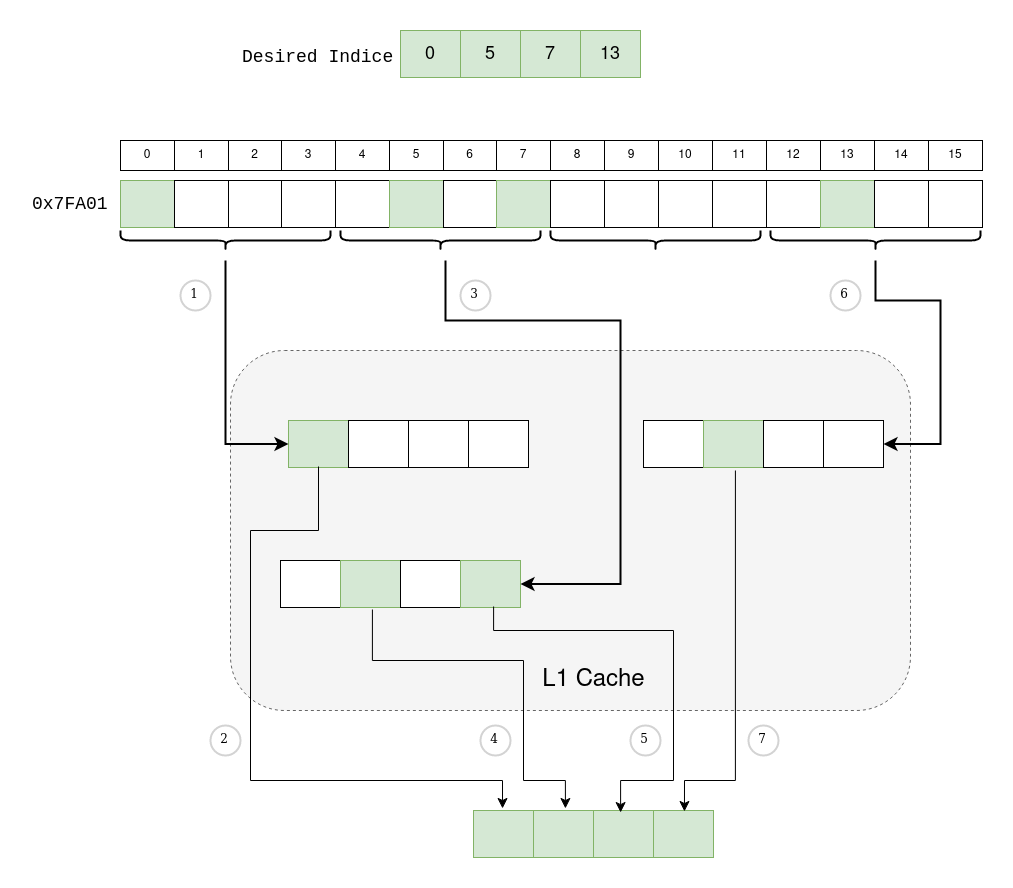
\includegraphics[width=\textwidth]{Figures/03-approach/Gather load.drawio.png}
\centering
\caption{ Order of Gather Load micro-operations: The effective address for all target elements is calculated in the floating point unit. Memory is divided into equally sized chunks, and they are moved to the cache. Corresponding element(s) are then extracted from the cache line and moved to the result vector.}
\label{fig:gather-load}
\end{figure*}

\rfig{gather-load} depicts micro-operations done to execute a \emph{single} gather load instruction. 
The processor first divides the array's memory space into equally sized chunks that fit into a cache line. Chunks that contain elements that are the target of the gather instruction are then moved to the cache. This requires calculating the memory address of each single element to be accessed. Address calculations are done in floating point operation pipeline \cite{A64FXmanual} which increases the latency. Once a cache line is brought into the cache, desired elements are extracted and moved to the result vector.

All these operations are done for executing a \emph{single} gather load instruction. There are two sources of performance degradation upon executing these operations:
\begin{inparaenum}
\item Latency of accessing different locations in the memory and bringing them into the cache and \item keeping floating point unit busy for address calculations.
\end{inparaenum}

The significant number of stalled cycles shown in \rtab{gather-scatter-bad} is a direct result of the first issue. Moreover, processors typically try to execute other none-memory-access instructions that do not depend on the result of the load instruction to avoid stalls while waiting for the memory operations to finish however, for the gather load instruction, keeping floating point unit busy due to address calculations would disable the processor to do so, resulting in significant stalled cycles even if the loop contains many arithmetic instructions.


When Praharenka \etal evaluated their design, they had no access to hardware and thus based their evaluation on counting the number of instructions executed in a simulator.
\rtab{gather-scatter-bad} are the first results, obtained in real hardware with SVE, that show that the reduction in the number of instructions enabled by Praharenka \etal's \ALC design does not translate into faster execution.
Therefore, for an \ALC design to have a chance at being faster than \ifconverted and vectorized code, gather/scatter instructions need to be avoided or eliminated.
\rsec{alc-data-permutation} discusses how gather instructions can be eliminated.
\rsec{eval-scatters-costs} shows empirical results which indicate that reducing the number of scatter stores also improves ALC's performance.

\section{Efficient ALC via Data Permutation}
\label{sec:alc-data-permutation}


\begin{figure*}[t]
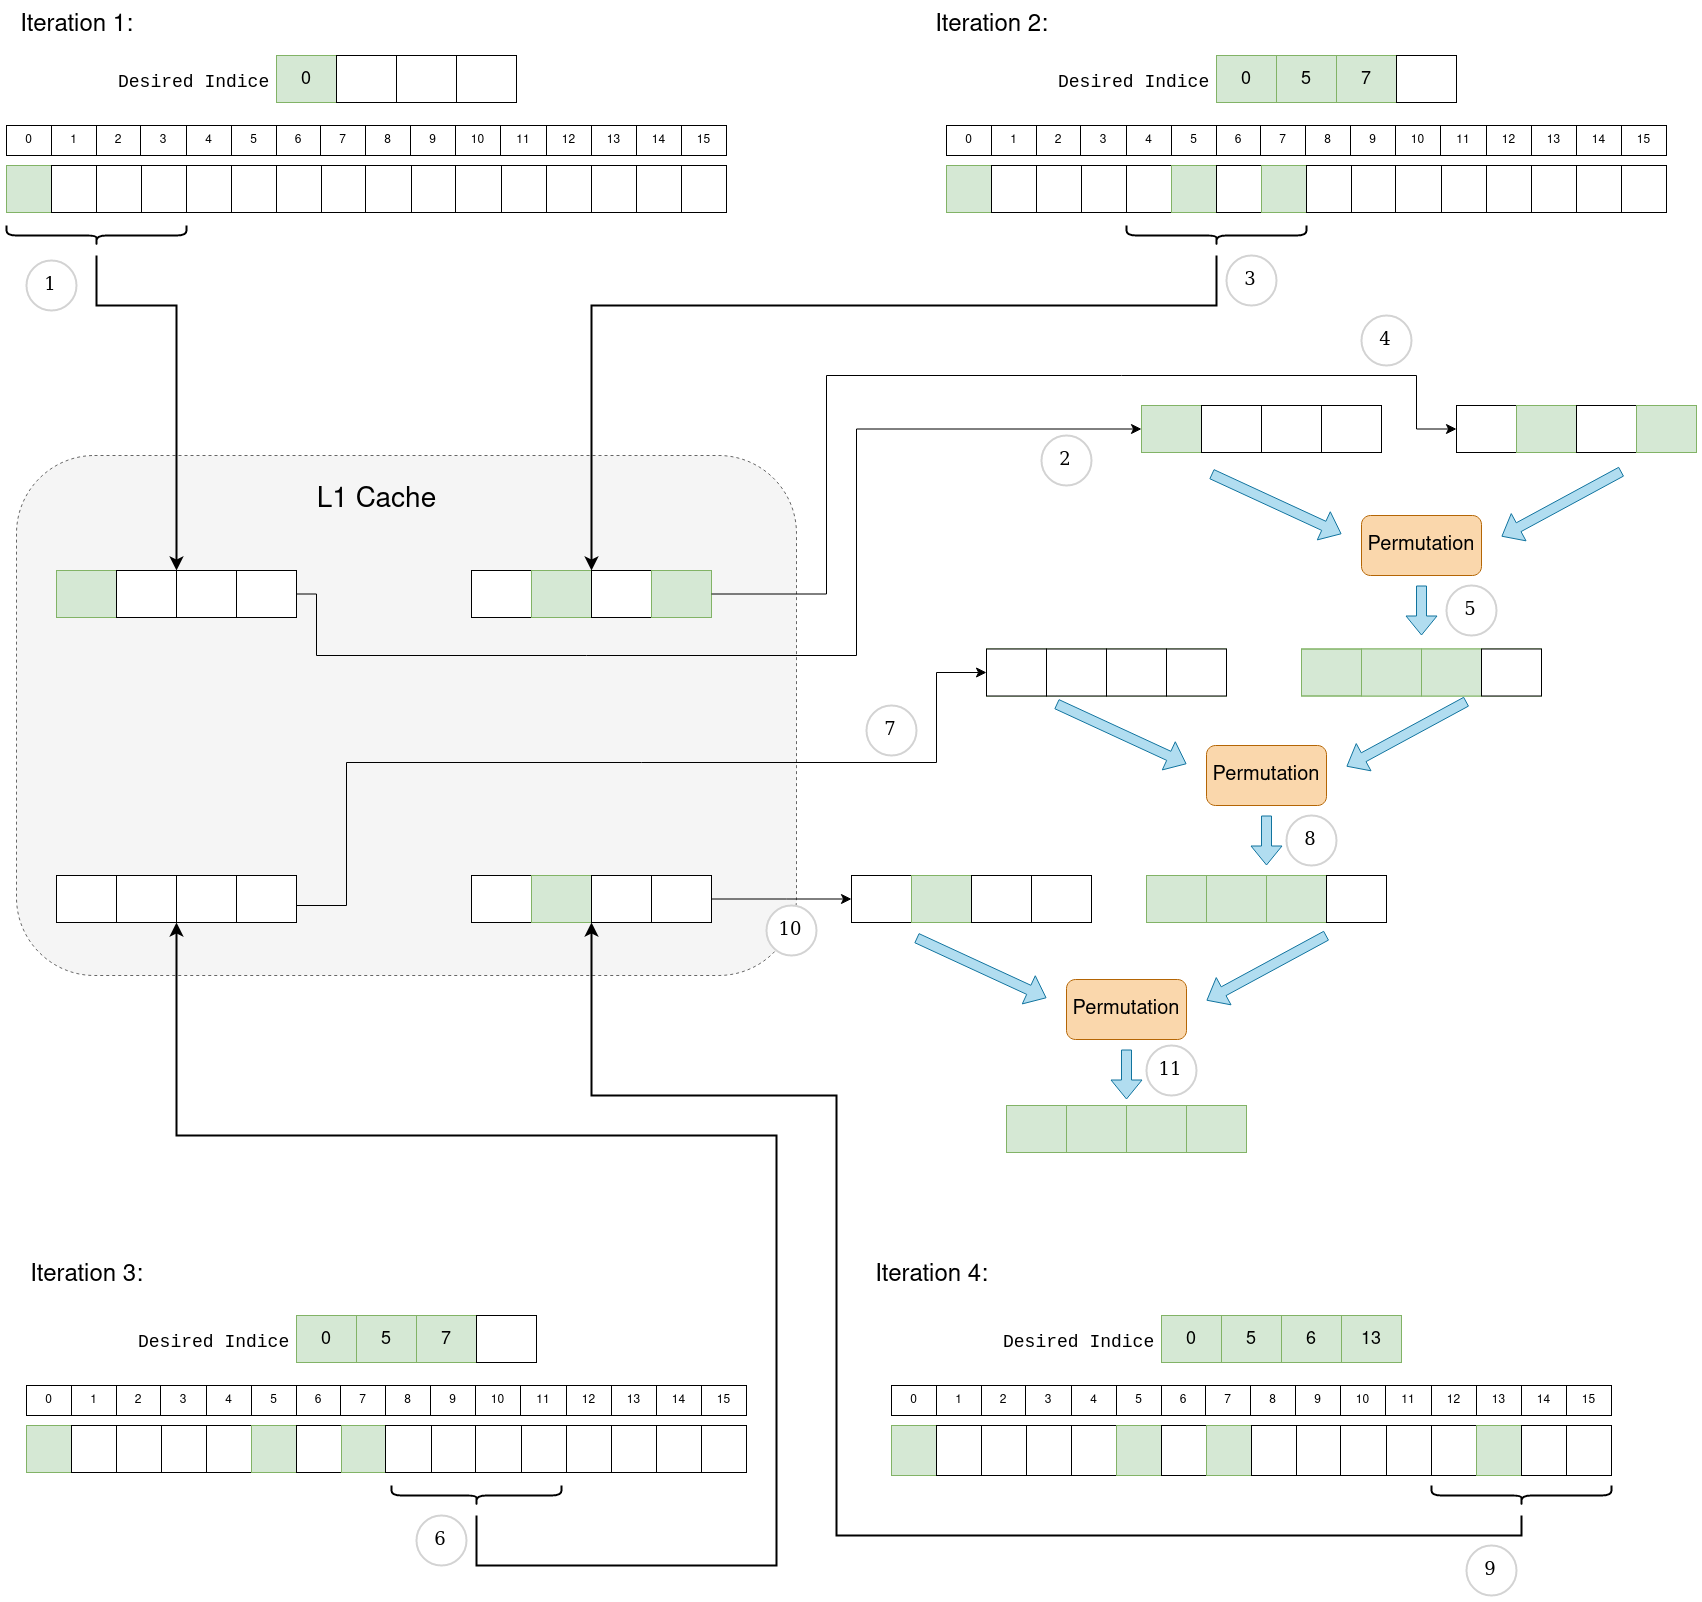
\includegraphics[width=1.1\textwidth, height= 14cm]{Figures/03-approach/Data_Permutation.drawio.png}
\caption{Data Permutation}
\label{fig:data-permutation}
\end{figure*}

Permuting both the indices and data vectors eliminates gather instructions.
\rfig{data-permutation} shows how gather load instructions discussed in \rfig{gather-load} can be broken into multiple regular vector-load instructions, from different loop iterations, and how the final result vector can be formed through permuting loaded data.

Data permutation and index permutation happen \emph{simultaneously}. This means that all indices that need to be loaded are not known initially, but as we iterate the vector loop, we find the indices we need to load. This can be seen in the figure where in each iteration, \emph{Desired Indices} is filled gradually. 

\circled{1} Initially, the first four elements are loaded into the cache and \circled{2} then transferred to a vector register, knowing that only the first element is desired. \circled{3}, \circled{4} Next iteration loads the next four elements to another vector register, which now contains two desired elements. \circled{5} These two loaded vectors are then permuted. The resulting register has three elements of those we are looking for. \circled{5}, \circled{6}, \circled{7} The third iteration loads a vector of elements whose elements are not desired so after the permutation, \circled{8} we obtain the same resulting vector. Finally, \circled{9}, \circled{10} the last four elements are loaded and undergo permutation, \circled{11} resulting in a vector filled with desired elements.

Replacing gather loads with data permutation could improve performance in several ways: 
\begin{inparaenum}[(i)]
  \item All load instructions now load from consecutive memory addresses, thus removing the need to compute an address for each element and allowing the processor to execute other instructions while waiting for the data to be transferred from memory because the floating-point unit is no longer busy with address computations. 
  \item The latency of each load is significantly smaller because it is served from a single cache line.
  \item The processor can effectively utilize prefetching and take advantage of spatial locality because it loads from consecutive addresses.
\end{inparaenum}


\begin{figure*}[htbp]
\centering
\begin{subfigure}[b]{0.31\textwidth}
\begin{lstlisting}[escapechar=|,language=PretendAsm, basicstyle=\fontsize{8}{12}\selectfont]
vload    v1, r1 ----->>
vload    v2, r2 ----->>
vload    v3, r3 ----->>
vcmp_lt  pT, v1, v2 -->>
vcmp_le  pF, v1, v2












vadd     v1, v1, v3, pF
vstore   v1, r1, pF




vmul     v2, v2, v3, pT
vstore   v2, r1, pT
br LATCH
\end{lstlisting}
\caption{\ifconv.}
\label{fig:simple-loop-ifconv}
\end{subfigure}%
\begin{subfigure}[b]{0.35\textwidth}
\begin{lstlisting}[escapechar=|,language=PretendAsm, basicstyle=\fontsize{8}{12}\selectfont]
// --------------->>
// --------------->>
// --------------->>
// --------------->>




# Index vector permutation.
permute vI, vM, vR, pT, pF ->
if_all_true vM, U_THEN -->>
# if vM is not uniform true,
# then vR is uniform false.
swap    vM, vR ------->>
U_ELSE:
gather  v1, r1, vM
gather  v3, r3, vM
vadd    v1, v1, v3
scatter v1, r2, vM ------>>
br LATCH
U_THEN:
gather  v1, r1, vM
gather  v3, r3, vM
vmul    v2, v2, v3
scatter v2, r1, vM ------>>
br LATCH
\end{lstlisting}
\caption{\ALC.}
\label{fig:simple-loop-alc}
\end{subfigure}
\begin{subfigure}{0.33\textwidth}
\begin{lstlisting}[escapechar=|,language=PretendAsm, basicstyle=\fontsize{8}{12}\selectfont]
//
//
//
//
# Data vector permutation.
permute v1, v1M, v1R, pT, pF |\label{lst:alc-dp-a}|
permute v2, v2M, v2R, pT, pF |\label{lst:alc-dp-b}|
permute v3, v3M, v3R, pT, pF |\label{lst:alc-dp-c}|
//
//
//
//
//
//
U_ELSE:
# No need to gather a or
# c as data is permuted.
vadd    v1, v1R, v3R
//
br LATCH
U_THEN:
# No need to gather b or
# c as data is permuted.
vmul    v2, v2M, v3M
//
br LATCH
\end{lstlisting}
\caption{\ALCdp.}
\label{fig:simple-loop-alc-dp}
\end{subfigure}

\caption{Main loop blocks generated when compiling \rlst{simple-loop} vectorization approach. In all three versions, \code{r1}, \code{r2}, and \code{r3} are pointer registers, advanced on each iteration in the loop's \code{LATCH} block (not shown), to array $a$, $b$, and $c$ respectively. In both (b) and (c), \code{vI} is the \emph{index vector}, \code{vM} is the \emph{merge vector}, and \vR is the \emph{remainder vector}. Registers \code{vXM} and \code{vXR} are the merge and remainder vectors after permutation of vector register \code{X}. Instructions that are the same on different versions of the code are omitted --- indicated with ``\code{//}''.}
\label{fig:simple-loop-versions}
\end{figure*}


\rfig{simple-loop-versions} contrasts the differences in the code generated by the compiler from the example code in \rlst{simple-loop}.
In \rfig{simple-loop-alc} the data for both consolidated paths are loaded with gather instructions and the permuted index vector \vM.
In contrast, \ALCdp eliminates gather instructions by also permuting  the data vectors (\code{v1}, \code{v2}, and \code{v3}), as \rlines{alc-dp-a}{alc-dp-c} in \rfig{simple-loop-alc-dp} shows.
As a result, \ALCdp benefits from the same spatial locality and data prefetching as the \ifconverted code (\rfig{simple-loop-ifconv}).
When \vM is not uniformly true, then it is guaranteed that \vR is uniformly false because there are only two \cpaths.
This observation allows the compiler to generate an optimized version of \iterALC where loads for the first iteration of the loop are peeled.
In \rfig{simple-loop-alc} and \rfig{simple-loop-alc-dp} \vM is initialized with the index vector of from the peeled iteration.
Similarly, vectors \code{v1M}, \code{v2M}, and \code{v3M} are initialized with the data loaded from $a$, $b$, and $c$ as in the first iteration of the \ifconverted \& vectorized loop (\rfig{simple-loop-ifconv}).
With the above optimization, most loop iterations operate with fully uniform vectors leading to better utilization of the SIMD units.

\rtab{gather-scatter-bad} shows that eliminating gather instructions via data permutation (\ALCdp) significantly improves the performance of ALC.
In particular, \ALCdp has over $5\times$ less stalled cycles and executes in $3.8\times$ fewer cycles than \ALC, even though it executes almost $4\times$ more instructions.
This result indicated that reducing the number of executed instructions does not necessarily translate into better performance.
Moreover, \ALCdp has over $84\times$ fewer stalls due to waiting for memory operations, as \rtab{gather-scatter-bad} shows.
Memory stalls are significantly reduced because data vectors are loaded from consecutive memory locations, which benefit from the higher spatial locality and more accurate prefetching.
On the other hand, gather instructions suffer from higher latencies in the address calculation and poor spatial locality of data elements.
Therefore, the results in \rtab{gather-scatter-bad} indicate that trading off the execution of more instructions with avoiding gather instructions pays off.
Data permutation adds vector-vector instructions, which have significantly lower latency than sophisticated memory instructions, such as gather/scatter instructions~\cite{A64FXmanual}.

\rtab{gather-scatter-bad} shows that \ALCdp does not perform better than \ifconv for the code in \rlst{simple-cond-copy-loop}.
There is little room for ALC to save cycles by not executing vector instructions with inactive lanes because the simple loop does not perform enough work.
ALC can only outperform \ifconversion \& vectorization on loops that have a sufficient number of instructions to hide the permutation overhead.
In addition, a more significant number of instructions on \cpaths translates to more saved cycles, and fewer executed instructions, for loops with mutually exclusive paths.

\section{Single Control-Flow-Dependent Path Case}
\label{sec:single-if-statement-approach}
\begin{figure*}[t]
  \centering
  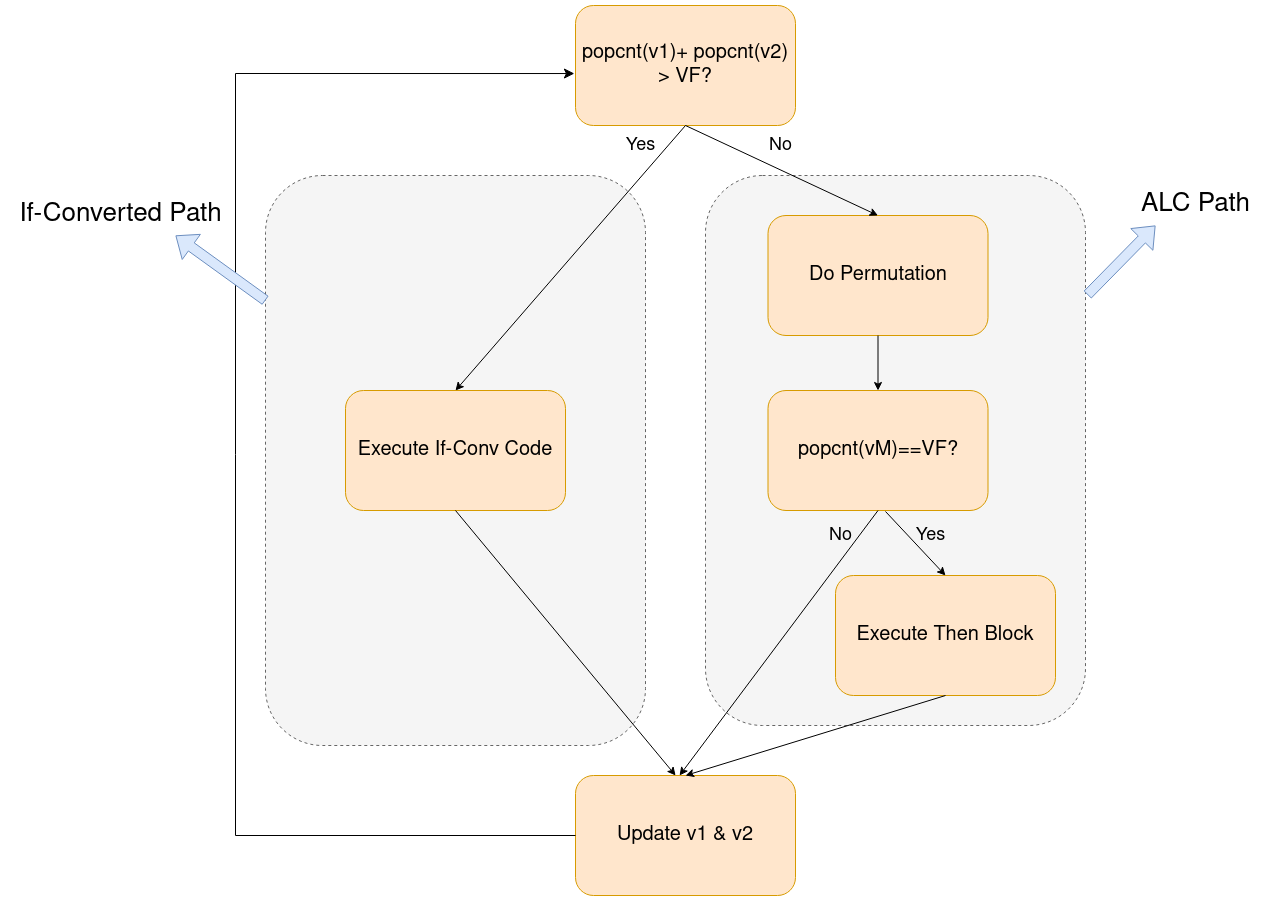
\includegraphics[width=\textwidth]{Figures/03-approach/single_if.png}
  \caption{Combining If-Conversion and ALC for the Single Control-Flow-Dependent Path Case: \code{v1} and \code{v2} are index vectors, and \code{popcount} is an  instruction that counts the number of true predicates for a given vector. The if-Conversion path is executed whenever the total number of active lanes is more than the \code{VF}(\emph{vector factor}) otherwise, ALC path is taken at runtime.}
  \label{fig:single-if}
\end{figure*}


Loops with a single \cpath, as the example in \rlst{simple-cond-copy-loop}, are a special case where the ALC design can be modified to extract the best of both \ifconversion and ALC.
In such loops, vector lanes are wasted with inactive elements, but the instructions on the single \cpath are the only source of wasted operations.
Therefore, \ifconversion \& vectorization is a good solution when the majority of lanes in the predicate vector are active, but in the complementary case --- loops with very sparse predicate vectors --- \ifconverted \& vectorized code executes a significant number of instructions that waste vector lanes.



With this in mind, the ALC algorithm needs to be modified such that it benefits from both permutation and \ifconversion.
Prior to index and data vector permutation, in each iteration, the number of active lanes can be calculated via population-count instructions that are available on most modern ISAs (e.g. ARMv8.2-A \& v9).
If there are more active elements than the \emph{vector factor} (VF) on \emph{both} index vector, then the \ifconverted code is executed, resulting in few wasted lanes.
Otherwise --- when there are fewer active lanes than VF --- an ALC path is executed where vectors are permuted and the consolidated-uniform path is executed when the predicate vector is uniform.
\rfig{single-if} shows a diagram which illustrates the approach.

Another benefit of combining ALC with if-conversion is a considerable reduction in permutation overhead. In the original algorithm for permutation, we needed to compute two vectors \vM and \vR and their corresponding predicate vectors. However, in this case \vR will be fully inactive because the vector permutation only happens when fewer than VF lanes are active. 
Therefore, there is no need for the compiler to emit instructions to produce \vR and its predicate vector.

\rfig{new-permutation} presents the new permutation algorithm. The inputs to the algorithm are two vectors with their corresponding predicate vector, where we know that \emph{the total number of active elements in both vectors are less than the VF}. After Permutation, there will be a Merge vector (\code{vM}) containing the consolidated active elements and its corresponding predicate vector (\code{pM}).
The new Permutation algorithm results in reduction in instruction overhead of the permutation logic by $50\%$. 

\begin{figure*}[h]
\begin{lstlisting}[escapechar=|,language=PretendAsm, basicstyle=\fontsize{12}{14}\selectfont, style=code_snippet_style]
# v0: first index vector
# v1: second index vector
# p0: first predicate vector
# p1: second predicate vector
# vM: resulting index vector
# pM: resulting predicate vector


|\color{blue}compact|  |\color{black}v2, v0, p0| 
|\color{blue}compact|  |\color{black}v3, v1, p1|
|\color{blue}cntp|       |\color{black}x0, p1, p1|
|\color{blue}cntp|       |\color{black}x1, p2, p2|
|\color{blue}add|        |\color{black}x2, x0, x1|
|\color{blue}whilelt|    |\color{black}p3, wzr, x0|
|\color{blue}splice |    |\color{red}vM||\color{black}, v2, v3, p3|
|\color{blue}whilelt|    |\color{red}pM||\color{black}, wzr, x2|
\end{lstlisting}
\caption{Permutation algorithm for Single Control-Flow-Dependent Path case using SVE vector instructions.}
\label{fig:new-permutation}
\end{figure*}




